\chapter{Amplificadores Operacionales. }\label{operacionales}

\hspace{10pt} El amplificador operacional monolítico (AO), es el tipo de circuito integrado más ampliamente conocido e utilizado en el diseño en
electrónica analógica. Desde su introducción en el mercado en la
década de 1960, los AOs se encuentran presentes en los más diversos diseños de sistemas electrónicos.

En este capítulo se estudiarán algunas de las más importantes
aplicaciones de los amplificadores operacionales; tanto en circuitos
lineales como no lineales. También se dará una visión general de las
características reales de funcionamiento y propiedades de los AOs.
%\def\baselinestretch{1.66}

%%% ----------------------------------------------------------------------

\section{Amplificadores operacionales ideales}

\hspace{10pt} Un amplificador operacional ideal es un amplificador diferencial de
tensión con una ganancia de tensión $a_v \rightarrow \infty$, una
impedancia de entrada $R_i \rightarrow \infty$ y una impedancia de
salida $R_o \rightarrow 0$. En la figura \ref{ao1} se muestra el
diagrama esquemático de un AO ideal, es de notar que un amplificador
de estas característica puede tener una tensión de salida $v_o$
finita con una tensión de entrada $v_i \rightarrow 0$. También un AO
ideal debe tener un ancho de banda $BW\rightarrow\infty$, las
corrientes de entrada en ambos terminales deben ser nulas (debido a
la impedancia de entrada $\infty$) y la tensión de salida debe ser
nula (sin desajuste) cuando son nulas las tensiones de entrada.
Estas características ideales no se logran en los circuitos reales,
sin embargo este modelo simplificado puede utilizarse en muchas de
las aplicaciones, dentro de un rango de trabajo determinado, sin
cometer errores apreciables.

\begin{figure}
	\centering
	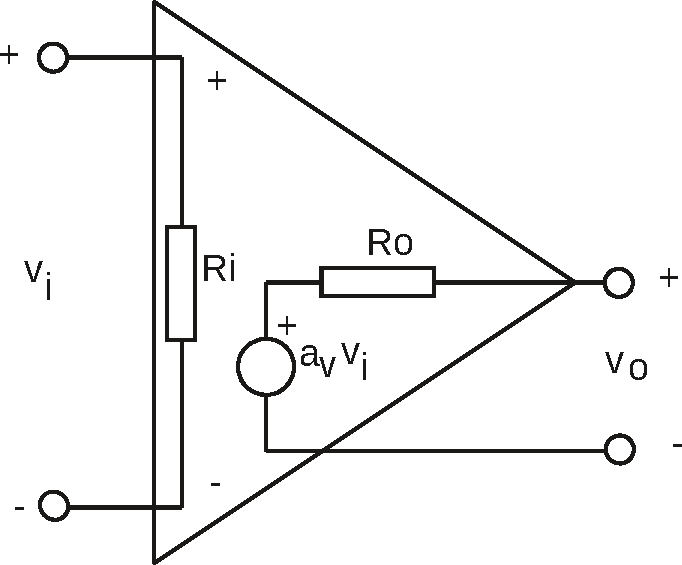
\includegraphics[width=2in]{figuras/ao1.pdf}\\
	\caption{Amplificador operacional ideal.}\label{ao1}
\end{figure}

En la mayor parte de las aplicaciones lineales los amplificadores
operacionales son utilizados como parte de un sistema realimentado. En la figura \ref{ao2} se muestran las dos
configuraciones circuitales más utilizadas con AOs: a) como
amplificador inversor, y b) como amplificador no inversor.

En la figura \ref{ao2} a) se puede deducir que $V^+=V^-=0$, debido a
que $I^-=0$ (impedancia de entrada del AO a lazo abierto
$\rightarrow \infty$). Por lo tanto $I_1=\frac{\displaystyle
	V_i}{\displaystyle R_1}$ y $V_o=-I_1 R_2$; de estas dos expresiones
se deduce que la ganancia de tensión realimentada es:
\begin{center}\label{ec1}
	\begin{equation}
		A_v=\frac{\displaystyle V_o}{\displaystyle
			V_i}=-\frac{\displaystyle R_2}{\displaystyle R_1}
	\end{equation}
\end{center}
; es decir un amplificador inversor. Estas expresiones son exactas
en el caso de un AO ideal, en donde una tensión $V_o$ finita puede
obtenerse a partir de una diferencia de potencial $V^+-V^-
\rightarrow 0$. En el caso real dicha diferencia de potencial no es
nula, aunque muy pequeña con respecto a $V_o$, por lo que a los
efectos prácticos muchas veces puede despreciarse y utilizar el
modelo de AO ideal. Debido al mismo efecto de diferencia de
potencial casi nula entre las entradas del AO el generador $V_i$
``ve`'' una impedancia igual a $R_1$.

\begin{figure}
	\centering
	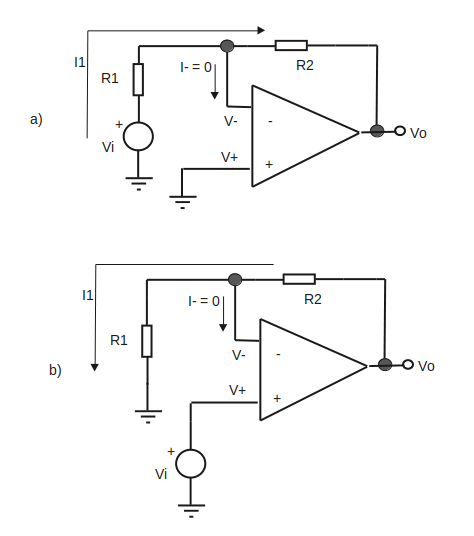
\includegraphics[width=3in]{figuras/ao2.png}\\
	\caption{Amplificador operacional ideal: a) configuración inversora; b) Configuración no inversora.}\label{ao2}
\end{figure}

En la figura \ref{ao2} b) $V_i=V^+=V^-$, $I_1=\frac{\displaystyle
	V_i}{\displaystyle R_1}$ y $V_o=I_1(R_1+R_2)$. Por lo tanto la
ganancia de tensión será:
\begin{center}\label{ec2}
	\begin{equation}
		A_v=\frac{\displaystyle V_o}{\displaystyle
			V_i}=1+\frac{\displaystyle R_2}{\displaystyle R_1}
	\end{equation}
\end{center}
; un amplificador no inversor con consideraciones parecidas a las
del caso anterior con respecto a la validez del modelo ideal. La
impedancia que ``ve'' el generador $V_i$ es muy alta
($\rightarrow\infty$ en el caso ideal).

Resumiendo, cuando se utiliza el modelo de AO ideal en un circuito
con realimentación negativa, se considera que $V^+=V^-$, que las
corrientes de entrada al AO son nulas y que la salida del
operacional se comporta como un generador de tensión ideal. En
muchas aplicaciones, y dentro de un rango de valores determinado,
este modelo sencillo puede ser utilizado; cuando este modelo no sea
suficiente para describir el funcionamiento se utilizan modelos más
elaborados que tienen en cuenta el carácter no ideal de los AOs.

\section{Amplificadores operacionales reales}

\subsection{Amplificadores operacionales como amplificadores de tensión reales}
\hspace{10pt} Si se toma al AO como un amplificador de tensión con características no ideales, un
primer modelo sería el de un amplificador diferencial con una
impedancia de entrada diferencial $Z_{id}$ no infinita, una
impedancia de salida $Z_o$ no nula y una ganancia de tensión $a_v$
finita. Una característica real adicional que se puede incorporar a
este primer modelo es una limitación en el rango dinámico de salida,
dado aproximadamente por las fuentes de alimentación generalmente
doble ($\pm V_{CC}$). En la figura \ref{ao3} se muestra: a) el diagrama
esquemático, b) la transferencia de dicho modelo real simplificado y
b) el modelo circuital.

\begin{figure}
	\centering
	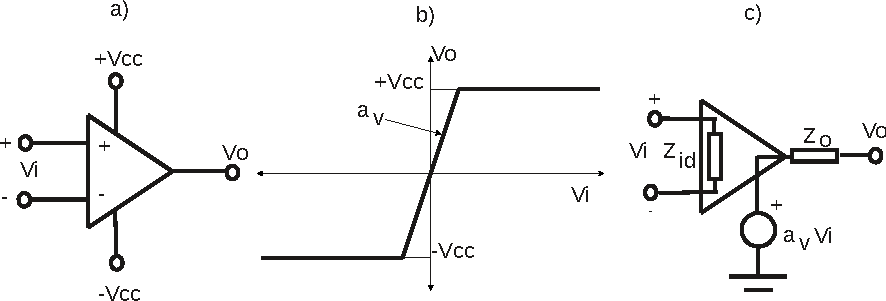
\includegraphics[width=5in]{figuras/ao3.pdf}\\
	\caption{Amplificador operacional como amplificador de tensión no ideal: a) diagrama esquemático, b) transferencia y c) circuito equivalente.}\label{ao3}
\end{figure}

Si se analiza la configuración no inversora de la figura \ref{ao2}
b) utilizando al AO como un amplificador de tensión real, se tiene
un circuito realimentado con una configuración serie-paralelo. La
red de realimentación $f$ está compuesta por las resistencias $R_1$
y $R_2$. En la figura \ref{ao4} se desarrolla la ganancia de tensión
realimentada $A=\frac{\displaystyle v_o}{\displaystyle v_i}$ por el
método de los cuadripolos. La transferencia de la red de
realimentación es $f=\frac{\displaystyle R_1}{\displaystyle
	R_1+R_2}$, por lo tanto si la ganancia de lazo $T \gg 1$, entonces
la ganancia realimentada será: $A \simeq \frac{\displaystyle
	1}{\displaystyle f}=1+\frac{\displaystyle R_2}{\displaystyle R_1}$,
coincidente con el desarrollo realizado para el AO ideal.

\begin{figure}
	\centering
	\includegraphics[width=5in]{figuras/ao4.png}\\
	\caption{Configuración no inversora.}\label{ao4}
\end{figure}

Como sabemos de la teoría de realimentación, la impedancia de
entrada realimentada se ve incrementada en $(1+af)$ con respecto a
la impedancia sin realimentar y la impedancia de salida tiende a
disminuir $(1+af)$ veces con respecto a la sin realimentar, es decir
lo acercan a un amplificador ideal si $af \gg 1$.

En forma similar se puede analizar la configuración inversora de la
figura \ref{ao2} a). Este amplificador realimentado pertenece a la
configuración de realimentación paralelo-paralelo siendo la
resistencia $R_2$ la red de realimentación $f$. En la figura
\ref{ao5} se realiza el cálculo de la ganancia de tensión utilizando
el método de cuadripolos, llegando también en este caso, que el
cálculo realizado con el modelo ideal y el real coinciden cuando $af
\gg 1 $.


\begin{figure}
	\centering
	\includegraphics[width=5in]{figuras/ao5.png}\\
	\caption{Configuración inversora.}\label{ao5}
\end{figure}


\subsection{Estructura interna de los amplificadores operacionales}

\hspace{10pt} Si bien no se estudiará en detalle la estructura y arquitectura
interna de los amplificadores operacionales, se dará una visión
general de ella que ayude a comprender algunas características
particulares.

La mayor parte de los AOs, sean de tecnología bipolar o CMOS, poseen
al menos tres etapas diferenciadas. La etapa de entrada es en
general un amplificador diferencial, con alta impedancia de entrada,
alto rechazo a las señales de modo común, bajas corrientes de
polarización y alta ganancia de tensión; las etapas intermedias son 
también de alta ganancia y la etapa de salida, generalmente clase B 
o AB de baja impedancia de salida. La mayoría de los AOs responden a una
configuración esquematizada en la figura \ref{ao6}, en la parte
superior se muestra el esquema general y en la inferior el circuito
simplificado.

La etapa de entrada es un amplificador diferencial formado por $Q_1$
y $Q_2$ y polarizado por la fuente de corriente $I_1$; los
colectores son conectados a la carga activa formada por los
transistores $Q_3$ y $Q_4$ que forman un ``espejo de corriente'',
brindándole una alta impedancia de modo que la etapa diferencial
presenta una alta ganancia de tensión. La etapa intermedia, formada
por los transistores $Q_5$ y $Q_6$, por la resistencia $R_1$ y
polarizada por $I_2$, es una etapa de ganancia en configuración
emisor común. La etapa de salida es un amplificador de ganancia
unitaria clase AB polarizado con la fuente de corriente $I_3$.

El capacitor $C_1$ de la figura mencionada realiza la compensación
por polo dominante del modo ya desarrollado en el punto
\ref{ejemplo1}, en el caso que el AO no sea compensado internamente
el circuito integrado suele tener disponibles los pines necesarios
para realizar la conexión externa del capacitor $C_1$. Los AO
compensados internamente están diseñados con un margen de fase de
$45°$ para realimentación unitaria, como por ejemplo el muy
utilizado amplificador operacional de propósitos generales $\mu
A741$.

El esquema circuital de los amplificadores operacionales reales
sugiere que otra de las características no ideales a tener en
cuenta, es la de la respuesta en frecuencia y la de su compensación
correspondiente; completando el modelo simplificado presentado en el punto anterior.


\begin{figure}
	\centering
	\includegraphics[width=5in]{figuras/ao6.png}\\
	\caption{Configuración esquematizada de un amplificador operacional básico.}\label{ao6}
\end{figure}

\subsection{Características de corriente continua}

\hspace{10pt} Un AO ideal es un amplificador que responde tanto a las señales de
continua como a las señales variables en el tiempo. Además su
tensión de salida $V_o$ será $0$ si su entrada diferencial $V_{i}=0$
y sus corrientes de entrada serán nulas debido a la impedancia de
entrada infinita.

En el caso real existe una tensión de salida no nula para $V_{i}=0$
y corrientes no nulas de polarización de entrada. En algunas de las
aplicaciones que utilizan AOs estos desajustes deberán ser tenidos
en cuenta, ya que pueden influir en su correcto funcionamiento.

\subsubsection{Desajuste de tensión}

\hspace{10pt} En la figura \ref{ao6} se aprecia que si los pares de transistores
$Q_1 - Q_2$ y  $Q_3 - Q_4$ son iguales y los transistores $Q_7$ y
$Q_8$ son perfectamente complementarios; se puede lograr, en el caso
ideal, que $V_o=0$ para $V_i=0$. En un circuito integrado real este
apareamiento de transistores se puede lograr de una manera eficiente
pero no totalmente equivalente; por lo que este desapareamiento hará
que $V_0 \neq 0$ para $V_i=0$. En la figura \ref{ao7} a) se muestra,
para una entrada diferencial simplificada, el efecto que producen
dos transistores no totalmente apareados; allí se ve que una
diferencia en las curvas de entrada de dichos transistores se
reflejará en un diferencia entre las corrientes de colector
respectivas, alejándose del valor ideal $I_{C1}=I_{C2}=I_1/2$. Esta
diferencia de corrientes se propagará en el circuito haciendo que la
salida $V_0\neq0$. Como este desapareamiento  depende de las
tolerancias producidas en el proceso de fabricación de los circuitos
integrados, los fabricantes sólo aseguran los extremos estadísticos
de variación de las curvas de sus transistores.

Para cuantificar esta variación se define la tensión de desajuste
$V_{OS}$ (\emph{off-set} en inglés): como la máxima tensión, en
valor absoluto, que debe colocarse a la entrada de un AO para que la
salida sea $V_o=0$; en la figura \ref{ao7} b) se esquematiza tal
situación, siendo $V_{OS}$ la tensión de entrada que asegura que
$V_o=0$ (en un esquema simplificado se igualan
$I_{C1}=I_{C2}=I_1/2$).

Para calcular el efecto de la tensión de desajuste $V_{OS}$ en un
circuito real se utiliza un modelo que consta de una fuente a la
entrada de valor absoluto $\mid V_{OS} \mid$ y un AO ideal. En la
figura \ref{ao8} se muestra un ejemplo de cálculo y su resultado. El
resultado debe interpretarse como los extremos de variación de la
tensión de salida debido a $V_{OS}$.

\begin{figure}
	\centering
	\includegraphics[width=3in]{figuras/ao7.png}\\
	\caption{Desajuste de tensión: a)$V_0\neq 0$ para $V_i=0$, b) tensión de desajuste de entrada $V_{OS}$ para asegurar $V_0=0$.}\label{ao7}
\end{figure}


\begin{figure}
	\centering
	\includegraphics[width=3in]{figuras/ao8.png}\\
	\caption{Cálculo de la tensión de desajuste de salida debido a $V_{OS}$.}\label{ao8}
\end{figure}

\subsubsection{Desajuste debido a las corrientes de polarización de entrada}

\hspace{10pt} En la entrada diferencial simplificada de la figura \ref{ao6} se ve que, aun en el caso de perfecto apareamiento, las
corrientes de polarización de los transistores $Q_1$ y $Q_2$ son no
nulas; debiéndose cerrar éstas en los circuitos externos y pudiendo
producir caídas de tensión que afecten a la tensión continua de
salida. Es de notar que en los AOs bipolares estás corrientes
(corrientes de base en un TBJ) serán mucho más apreciables que en un
AO CMOS (corrientes de pérdida en los \emph{gates}); pero en ambos
casos las corrientes tendrán un sentido definido por los
transistores utilizados; como en el caso de la figura \ref{ao6} en
el cual ambas corrientes serán entrantes.

En un primer análisis se supondrá un perfecto apareamiento;
siguiendo el esquema de la figura \ref{ao6} se ve que en estas
condiciones las corrientes de polarización de base serán iguales
($I_{B1}=I_{B2}=I_B$). El modelo que se utilizará para el cálculo
será el mostrado en la figura \ref{ao9} a); allí se ubican dos
generadores de corriente $I_B$ con la polaridad adecuada en cada una
de las entradas del AO, considerándolo a éste ideal para todos los
demás efectos. En la figura \ref{ao9} b) se muestra un ejemplo de
cálculo del desajuste de la tensión de salida $V_o$ debido a las
corrientes de polarización de entrada.

Si no existe un perfecto apareamiento entre $Q_1$ y $Q_2$, como en
un AO real, la corriente $I_B$ debe interpretarse como el promedio
estadístico de la corriente de polarización asegurado por el
fabricante. Es de notar que el efecto de la corriente promedio puede
anularse, como se muestra en la figura \ref{ao9} b), si
$R_3=R_1\|R_2$.

\begin{figure}
	\centering
	\includegraphics[width=4in]{figuras/ao9.png}\\
	\caption{Cálculo de la tensión de desajuste de salida debido a $I_B$; a) modelo a utilizar, b) ejemplo de cálculo.}\label{ao9}
\end{figure}

Para cuantificar la variación estadística de las corrientes de
polarización se define la corriente de desajuste de entrada:
$I_{OS}=I_{Bmax}-I_{Bmin}$, es decir la diferencia entre las
corrientes de polarización máxima y mínima que asegura el
fabricante. Si como se mencionó anteriormente interpretamos a $I_B$
como la corriente promedio: $I_B=\frac{\displaystyle
	I_{Bmax}+I_{Bmin}}{\displaystyle 2}$; podemos obtener de los
parámetros $I_B$ e $I_{OS}$, suministrados por los fabricantes, los
extremos de variación de las corrientes de polarización de entrada:

\begin{center}
\end{center}
\begin{eqnarray}
	\nonumber
	I_{Bmax} & = & I_B + \frac{\displaystyle I_{OS}}{\displaystyle 2} \\
	\nonumber
	I_{Bmin} & = & I_B - \frac{\displaystyle I_{OS}}{\displaystyle 2} \\\label{ec3}
\end{eqnarray}

El modelo completo que tiene en cuenta las corrientes de
polarización de entrada, es similar al mostrado en la figura
\ref{ao9} a), con la diferencia que las fuentes de corriente
agregadas tienen en cuenta el efecto de $I_B$ y el de la máxima
variación posible $I_{OS}$, es decir se reemplaza cada generador
$I_B$ por dos generadores $I_B^+$ e $I_B^-$ respectivamente en las
entradas $+$ y $-$ del AO. Resolviendo en este caso el circuito
ejemplo de la figura \ref{ao9} b) se obtiene la siguiente expresión:
\begin{center}
	\begin{eqnarray}
		\nonumber
		V_o & = & - I_B^+ R_3 (1+\frac{\displaystyle R_2}{\displaystyle R_1}) + I_B^- R_2\\
		\nonumber
	\end{eqnarray}
\end{center}
; si $R_3=0 \quad \Rightarrow \quad V_o=I_B^- R_2$ y si
$R_3=R_1\|R_2 \quad \Rightarrow \quad V_o=(I_B^- - I_B^+) R_2$.

\subsubsection{Modelo completo de desajuste}

\hspace{10pt} En la figura \ref{ao10} se muestra el modelo completo de desajuste
que tiene en cuenta el desajuste de tensión $V_{OS}$ , el de
corriente $I_{OS}$ y la corriente promedio de polarización $I_B$. De
dicha figura se puede obtener la expresión de la tensión de
desajuste de salida total aplicando superposición a cada generador
del modelo, dando como resultado:
\begin{center}
	\begin{eqnarray}
		\nonumber
		V_o & = & \pm V_{OS}(1+\frac{\displaystyle R_2}{\displaystyle R_1}) - I_B^+ R_3 (1+\frac{\displaystyle R_2}{\displaystyle R_1}) + I_B^- R_2\\
		\nonumber
	\end{eqnarray}
\end{center}
; a esta expresión se le calculan los extremos de variación máximo y
mínimo del siguiente modo:
\begin{center}
	\begin{eqnarray}
		\nonumber
		V_{omax} & = & +V_{OS}(1+\frac{\displaystyle R_2}{\displaystyle R_1}) - I_{Bmin} R_3 (1+\frac{\displaystyle R_2}{\displaystyle R_1}) + I_{Bmax} R_2\\
		\nonumber
		V_{omin} & = & -V_{OS}(1+\frac{\displaystyle R_2}{\displaystyle R_1}) - I_{Bmax} R_3 (1+\frac{\displaystyle R_2}{\displaystyle R_1}) + I_{Bmin} R_2\\
		\nonumber
	\end{eqnarray}
\end{center}
; siendo $I_{Bmax}$ e $I_{Bmin}$ las definidas en las ecuaciones
\ref{ec3}.

\begin{figure}
	\centering
	\includegraphics[width=4in]{figuras/ao10.png}\\
	\caption{Modelo completo para el cálculo de la tensión de desajuste de salida.}\label{ao10}
\end{figure}

La corriente promedio de polarización $I_B$, la corriente de
desajuste $I_{OS}$ y la tensión de desajuste $V_{OS}$ cambian con la
temperatura. Un circuito cuidadosamente diseñado para anular el
desajuste de la tensión de salida a $25°C$ puede no permanecer en
ese estado cuando la temperatura se eleva por ejemplo a $35°C$. Este
es el llamado corrimiento térmico (\emph{thermal drift}). Los
fabricantes de AOs expresan este corrimiento como un factor en
$nA/°C$ y en $\mu V/°C$ para los corrimientos térmicos de corriente
y de tensión respectivamente. Si se aproxima a estos corrimientos
como lineales se puede estimar la variación total de la tensión de
desajuste de salida para una determinada variación de la
temperatura.

\subsubsection{Circuitos para anular la tensión de desajuste de salida}

\hspace{10pt} Algunos amplificadores operacionales poseen pines de entrada
dedicados a compensar el desajuste. Esto se logra actuando sobre la
polarización de la etapa diferencial de entrada de modo de
modificarla levemente y obtener por medición el ajuste a cero
necesario. Como ejemplo de este tipo de compensación se muestra en
la figura \ref{ao11} a) lo recomendado por el fabricante en el AO
$\mu A741$, en dicho circuito se debe diseñar $R_3=R_1\|R_2$ de modo
de compensar a $I_B$ y colocar el resistor variable $R_4=100K$ de la
manera indicada para compensar los desajustes de signo incierto.

En las figuras \ref{ao11} b) y c) se muestran posibles circuitos
externos de compensación para amplificadores operacionales
utilizados en su configuración inversora y no inversora
respectivamente. En estos casos el cursor de los resistores
variables puede entregar tensiones negativas o positivas, según su
posición, de modo de asegurar el ajuste a cero.


\begin{figure}
	\centering
	\includegraphics[width=4in]{figuras/ao11.png}\\
	\caption{Compensación de la tensión de desajuste de salida: a) conexiones para anular desajuste en un $\mu A741$; circuitos compensadores para b) amplificador inversor y c) no inversor.}\label{ao11}
\end{figure}

\subsection{Rapidez de respuesta (\emph{Slew Rate})}

\hspace{10pt} Otra característica no ideal que se debe tener en cuenta en un AO es
la denominada rapidez de respuesta (o \emph{slew rate}). Este
fenómeno no lineal cuantifica la máxima velocidad de cambio de la
tensión en la salida que puede manejar un determinado AO, y está
definido como:
\begin{center}
	\begin{eqnarray}
		\nonumber
		SR & = & \frac{\displaystyle dV_o}{\displaystyle dt}\biggr |_{max} \\
		\nonumber
	\end{eqnarray}
\end{center}
y por lo general está especificado en la hoja de datos en unidades
de $V/\mu seg$.

Para evaluar la distorsión no lineal que provoca se utilizará un AO
con ganancia de tensión a lazo abierto $a_o$ y compensado por polo
dominante a una frecuencia $w_1$. En forma aproximada se puede
suponer que se comporta como un amplificador de un polo con la
siguiente transferencia en el plano $s$:
\begin{center}
	\begin{eqnarray}
		\nonumber
		a(s) & = & \frac{\displaystyle a_o}{\displaystyle (1+\frac{\displaystyle s}{\displaystyle w_1})}\\
		\nonumber
	\end{eqnarray}
\end{center}
; si a este AO lo realimentamos en forma unitaria (ver figura
\ref{ao12}), se obtendrá un seguidor con la siguiente transferencia:
\begin{center}
	\begin{eqnarray}
		\nonumber
		A(s) & = & \frac{\displaystyle 1}{\displaystyle (1+ \frac{\displaystyle s}{\displaystyle w_f})}\\
		\nonumber
	\end{eqnarray}
\end{center}
; donde $w_f=w_1(1+a_o)$.

Si le aplicamos un escalón de tensión en
la entrada $V_i(t)=V_x \mu(t)$, la respuesta teórica debería ser de
la forma $V_o(t)=V_x(1-e^{-tw_f})$; sin embargo mientras la
pendiente de la expresión teórica de la salida se mantenga mayor que
el $SR$ del AO, éste sólo podrá variar su salida en forma lineal y a
la máxima velocidad posible , es decir el $SR$, en la figura
\ref{ao13} a) se muestra esta situación. De forma similar si
aplicamos a la entrada una onda senoidal de una frecuencia dentro
del ancho de banda del circuito, deberíamos obtener una réplica de
la señal a la salida debido a que el circuito del ejemplo se
comporta como un seguidor; sin embargo puede ocurrir que la
pendiente de la onda senoidal supere al $SR$, produciéndose una
distorsión no lineal (ver figura \ref{ao13} b).


\begin{figure}
	\centering
	\includegraphics[width=4in]{figuras/ao12.png}\\
	\caption{Transferencia de un circuito seguidor.}\label{ao12}
\end{figure}


\begin{figure}
	\centering
	\includegraphics[width=4in]{figuras/ao13.png}\\
	\caption{Respuesta de un seguidor actuando el SR: a) respuesta al escalón, b) respuesta a una onda senoidal.}\label{ao13}
\end{figure}

Para comprender en forma cualitativa el por qué de esta limitación
en la máxima velocidad de variación de la tensión de salida; se
puede analizar el circuito simplificado de la figura \ref{ao6} en su
parte superior; allí se puede observar que la tensión de salida
sigue aproximadamente a la tensión el capacitor de compensación
$C_1$ no pudiendo variar por lo tanto en forma instantánea, una
variación en la entrada se verá reflejada entonces totalmente en la
entrada diferencial del AO. La etapa diferencial se comporta en
forma lineal sólo para pequeños valores de su tensión de entrada
diferencial, cuando se la sobreexcita no se comporta en forma lineal
saturándose en corriente y entregando una corriente constante a la
siguiente etapa. Esta corriente constante es la que cargará al
capacitor $C_1$ en forma lineal (ver figura \ref{ao13}) hasta que la
velocidad de variación teórica de la salida baje lo suficiente para
que la entrada diferencial trabaje nuevamente en la zona lineal.

\subsection{El amplificador operacional real. Análisis de su hoja de datos.}

\hspace{10pt} El amplificador operacional ideal es una muy buena herramienta para
ilustrar las propiedades básicas de las aplicaciones que utilicen
AOs reales. Sin embargo en muchos casos el comportamiento de los
circuitos reales puede desviarse significativamente del predicho en
forma ideal. Algunas características no ideales de los AOs ya fueron
presentadas en los puntos anteriores.

Las principales características y parámetros eléctricos
suministrados por los fabricantes son enumerados a continuación,
tomando como base los datos del amplificador operacional de
propósitos generales $\mu A 741C$ de \emph{Texas Instruments}:

\begin{itemize}
	\item \textbf{Tensión de desajuste de entrada $V_{OS}$.} Ya
	definida anteriormente. Valor máximo en $\mu A 741C$ 6mV.
	\item \textbf{Corriente de desajuste de entrada $I_{OS}$.} Ya
	definida anteriormente. Valor máximo en $\mu A 741C$ 200nA.
	\item  \textbf{Corriente de polarización de entrada $I_B$.} Ya
	definida anteriormente. Valor máximo en $\mu A 741C$ 500nA.
	\item \textbf{Resistencia de entrada $r_i$.} Resistencia
	diferencial de entrada vista desde uno de los terminales de
	entrada con el otro a masa. Valor típico en $\mu A 741C$  $2M\Omega$.
	\item \textbf{Capacidad de entrada $C_i$.} Es la capacidad
	equivalente que se puede medir en  cualquier terminal de entrada
	con el otro termina a masa. Valor típico en $\mu A 741C$ 1,4pF.
	\item \textbf{Relación de rechazo al modo común $CMRR$.}
	Relación entre la ganancia en modo diferencial y la ganancia en
	modo común. Valor típico en $\mu A 741C$ 90dB.
	\item \textbf{Ganancia de tensión de gran señal $A_{VD}$.}
	Ganancia de tensión a lazo abierto a bajas frecuencias. Valor típico en $\mu A 741C$ 200 V/mV.
	\item \textbf{Respuesta en frecuencia.} Se definen, la frecuencia del polo
	dominante $f_1$ y la frecuencia de $0 dB$ $f_2$ a lazo abierto. Valores típicos en $\mu A
	741C$; $f_1=5Hz$ y $f_2=1Mhz$.
	\item \textbf{Resistencia de salida $r_o$.} Valor típico en $\mu A 741C$  $75 \Omega$.
	\item \textbf{Respuesta transitoria.} El tiempo de subida ($t_r$) y el
	sobreimpulso (\emph{Overshoot factor}) de una respuesta al escalón de un circuito de
	prueba utilizando al AO como seguidor. Valores típicos en $\mu A 741C$, $t_r=0,3 \mu seg$ y 3\% de
	sobreimpulso; en un seguidor cargado con una resistencia
	$R_L=2k\Omega$ en paralelo con una capacidad $C_L=100 pf$ con
	un escalón a la entrada de amplitud $20 mV$.
	\item \emph{\textbf{Slew Rate.}} Ya definido anteriormente. Valor típico en $\mu A 741C$ $0,5V/\mu seg$.
\end{itemize}


\section{Aplicaciones de amplificadores operacionales}

\hspace{10pt} Los amplificadores operacionales son ampliamente utilizados en
electrónica analógica. Las aplicaciones son innumerables, tanto en
circuitos lineales como no lineales. A continuación  se
desarrollarán algunas de las más importantes,  buscando
abarcar la mayor parte de sus aplicaciones básicas.

Para analizar el funcionamiento se utilizará, en
principio, el modelo ideal de AO; utilizando las características
reales en los casos necesarios.


\subsection{Aplicaciones operacionales básicas}

\subsubsection{Inversor con cambio de escala}

\hspace{10pt} En la figura \ref{ao14} a) se muestra el circuito correspondiente a
la configuración inversora. Allí la transferencia será:
$$A=\frac{\displaystyle v_o}{\displaystyle v_i}=-\frac{\displaystyle
	R_2}{\displaystyle R_1}$$, es decir un inversor con el
correspondiente cambio de escala. $R_3$ se coloca para compensar la
corriente promedio de polarización $I_B$ y debe ser igual a
$R_1||R_2$, como ya se explicó anteriormente.

\subsubsection{Amplificador no inversor con cambio de escala}

\hspace{10pt} Corresponde a la configuración no inversora y el circuito se muestra
en la figura \ref{ao14} b). Este amplificador posee una ganancia
dada por: $$A=\frac{\displaystyle v_o}{\displaystyle
	v_i}=1+\frac{\displaystyle R_2}{\displaystyle R_1}$$, con una
elevada impedancia de entrada, siendo las consideraciones para el
diseño de $R_3$ idénticas al caso anterior.

Un caso particular de esta configuración es el \textbf{seguidor de
	tensión}, mostrado en la fig \ref{ao14} c), en este caso la ganancia
será $A=1$; este circuito se comporta como un seguidor de tensión
alimentando una carga $R_L$ con una baja impedancia de salida y
presentando al generador de entrada una alta impedancia de entrada.

\begin{figure}
	\centering
	\includegraphics[width=4in]{figuras/ao14.png}\\
	\caption{Aplicaciones básicas de AOs: a) amplificador inversor, b) amplificador no inversor y c) seguidor.}\label{ao14}
\end{figure}

\subsubsection{Sumador ponderado}

El circuito de la figura \ref{ao15} es un sumador ponderado, con
salida invertida. La corriente en cada rama $i=1,2,\cdots,n$ será
$i_i=\frac{\displaystyle v_i}{\displaystyle R_i}$, por lo que la
corriente total sobre la $R_x$ será: $$i_x=\sum_{i=1}^n i_i$$; de
este modo la salida valdrá: $$v_o=-R_x \sum_{i=1}^n
\frac{\displaystyle v_i}{\displaystyle R_i}$$ Particularmente si
$R_1=R_2=\cdots=R_n=R_x$ el circuito se comportará como un sumador
puro con inversión.

\begin{figure}
	\centering
	\includegraphics[width=3in]{figuras/ao15.png}\\
	\caption{Sumador ponderado con inversión.}\label{ao15}
\end{figure}

\subsubsection{Restador (amplificador diferencial)}

\hspace{10pt} El amplificador diferencial más sencillo que utiliza operacionales
es el mostrado en la figura \ref{ao16}. De allí se puede obtener en
forma directa la expresión de la tensión de salida aplicando el
teorema de superposición dando como resultado:
$$v_o=-\frac{\displaystyle R_2}{\displaystyle R_1} v_1 + \frac{\displaystyle R_2}{\displaystyle  R_2+R_1}(1+\frac{\displaystyle R_2}{\displaystyle R_1})v_2=\frac{\displaystyle R_2}{\displaystyle R_1}(v_2-v_1)$$
La ganancia de este circuito depende de las resistencias $R_1$ y
$R_2$. En los amplificadores diferenciales suelen ser muy
importantes las características de rechazo al modo común e
impedancia de entrada. En este circuito la relación de rechazo al
modo común depende del grado de apareamiento de las resistencias
supuestas iguales en el circuito y la impedancia que se presenta a
las entradas son relativamente bajas y desbalanceadas, otro
inconveniente es que si se quiere ajustar la ganancia deberá
actuarse sobre dos de las resistencias simultáneamente, agravando el
desapareamiento.

Una posible solución a algunos de estos problemas se muestra en el
circuito de la figura \ref{ao17}, denominado \textbf{amplificador de
	instrumentación}, de este circuito se puede deducir que:
$$v_o=(1+\frac{\displaystyle 2 R_3 }{\displaystyle R_1})(v_2-v_1)$$

En este circuito el rechazo al modo común sigue dependiendo del
apareamiento de las resistencias, algo inevitable en este tipo de
circuitos. En cambio, la impedancia de entrada es elevada y
balanceada y la ganancia puede ser ajustada variando la resistencia
$R_1$, que es única, siendo su principal desventaja la utilización
de tres AOs.

\begin{figure}
	\centering
	\includegraphics[width=3in]{figuras/ao16.png}\\
	\caption{Amplificador diferencial.}\label{ao16}
\end{figure}

\begin{figure}
	\centering
	\includegraphics[width=3in]{figuras/ao17.png}\\
	\caption{Amplificador de instrumentación.}\label{ao17}
\end{figure}

\subsubsection{Integrador}

\hspace{10pt} En el circuito de la figura \ref{ao18} a) se puede obtener la
expresión de la tensión de salida $v_o(t)$ en función de $v_i(t)$,
ésta se halla sabiendo que $i(t)=\frac{\displaystyle
	v_i(t)}{\displaystyle R_1}$ y por lo tanto: $$\frac{ \displaystyle
	v_i}{\displaystyle R_1}=-C_f \frac{\displaystyle dv_o}{\displaystyle
	dt}$$ ; de aquí integrando en ambos miembros se obtiene:
$$v_o(t)=-\frac{\displaystyle 1}{\displaystyle R_1C_f}\int_o^tv_i(t)dt+v_o(0)$$
; por lo tanto la tensión de salida $v_o(t)$ será la integral,
cambiada de signo, de la tensión de entrada $v_i(t)$, siendo
$v_o(0)$ la condición inicial.

Hallando la transferencia de este circuito en el plano $s$ se
obtiene: $$A(s)=\frac{\displaystyle V_i(s)}{\displaystyle
	V_o(s)}=-\frac{\displaystyle 1}{\displaystyle sR_1C_f}$$, es decir
un integrador. A la derecha de la figura \ref{ao18} a) se muestra el
diagrama de amplitud de Bode de $A(jw)$.

El integrador mencionado puede traer algunos problemas prácticos
debido a que las corrientes de desajuste de continua, si bien
pequeñas, deberán cerrarse en parte por el capacitor $C_f$
produciendo un aumento progresivo en su tensión de continua pudiendo
llevar a la saturación al AO. Para evitar este efecto se coloca una
resistencia $R_f$ en paralelo con el capacitor $C_f$ de modo de
brindarle a las corrientes de polarización una camino de continua,
llegando a un valor constante como tensión de desajuste sobre el
capacitor $C_f$. Este integrador práctico se muestra en la figura
\ref{ao18} b), allí $R_c$ es la resistencia de compensación de la
corriente promedio de polarización $I_B$ y debe diseñarse como
$R_c=R_1||R_f$. La transferencia de este circuito práctico será
ahora: $$A(s)=- \frac{\displaystyle \frac{\displaystyle
		R_f}{\displaystyle R_1}}{\displaystyle 1+sC_fR_f}$$, y su diagrama
de amplitud se muestra a la derecha de la figura mencionada; el
circuito se comportará como integrador en la zona de frecuencias
donde la pendiente sea de $20 db/dec$. En forma práctica si
diseñamos a $R_f=10R_1$ podremos asegurar un funcionamiento como
integrador, casi sin diferencias con el ideal, a frecuencias
$w>\frac{1}{C_fR_1}$ (ver figura \ref{ao18} b)).

\begin{figure}
	\centering
	\includegraphics[width=4in]{figuras/ao18.png}\\
	\caption{Integrador: a) ideal, b) real.}\label{ao18}
\end{figure}

Existen otras configuraciones circuitales posibles de integradores,
entre ellas podemos mencionar a la mostrada en la figura \ref{ao19},
este circuito se comporta como un integrador sin inversión. En dicho
circuito podemos suponer $v_c(t)=v^+(t) \cong
v^-(t)=\frac{\displaystyle v_o(t)}{\displaystyle 2}$; con estas
consideraciones podemos plantear la ecuación nodal:
$$i_c(t)+\frac{\displaystyle v_c(t)-v_i(t)}{R}+\frac{\displaystyle
	v_c(t)-2v_c(t)}{R}=0$$; de lo que se deduce que:
$$i_c(t)=\frac{\displaystyle v_i(t)}{\displaystyle R}$$,
es decir que para cualquier carga $Z_L$ colocada en el lugar del
capacitor el circuito se comporta como una \textbf{fuente de corriente
	referida a masa}  dependiente de la entrada $v_i(t)$.
Particularmente en este caso, si se coloca una capacitor la tensión
$v_o(t)$ será: $$v_o(t)=2v_c(t)=\frac{\displaystyle 2}{\displaystyle RC}\int_0^t
v_i(t)dt+2v_c(0)$$; es decir un integrador. La transferencia en el
plano $s$ será: $$A(s)=\frac{\displaystyle V_o(s)}{\displaystyle
	V_i(s)}=\frac{\displaystyle 2}{\displaystyle
	sCR}$$

\begin{figure}
	\centering
	\includegraphics[width=3in]{figuras/ao19.png}\\
	\caption{Integrador no inversor.}\label{ao19}
\end{figure}

\subsubsection{Derivador}

\hspace{10pt} Si en el circuito integrador de la figura \ref{ao18} se invierten
capacitor y resistencia se obtiene un circuito cuya transferencia en
el plano $s$ es $A(s)=-sCR$, es decir un derivador. En la figura
\ref{ao20} se muestra el circuito ideal, allí la corriente sobre el
capacitor en función del tiempo es $i_c(t)=C\frac{\displaystyle
	dv_i}{\displaystyle dt}$; y la tensión de salida:
$$v_o(t)=-RC\frac{\displaystyle dv_i}{\displaystyle dt}$$; este
circuito teórico puede tener problemas de inestabilidad, debido a
que se agrega un polo en la ganancia de lazo $T(s)$ en
$f_p=\frac{\displaystyle 1}{\displaystyle 2 \pi RC}$, y puede ser
sensible a ruido de alta frecuencia debido a que su ganancia aumenta
a medida que aumenta la frecuencia.

Estos inconvenientes pueden salvarse agregando una resistencia $R_1$
en serie con el capacitor (ver figura \ref{ao21} a)). Tal
resistencia, en general tiene la característica de ser $<<R$ y
agrega un cero adicional a la ganancia de lazo $T(s)$ de modo de
compensarlo, y adicionalmente limita la ganancia a frecuencias altas
a $A=-\frac{\displaystyle R}{\displaystyle R_1}$. Por ejemplo si el
AO es un $\mu A741$ su ganancia a lazo abierto se puede aproximar a:
$$a(jw)=\frac{\displaystyle 200000}{(1+\frac{\displaystyle jf}{\displaystyle 5Hz})(1+\frac{\displaystyle jf}{\displaystyle
		1MHz})}$$; si $R=1K\Omega$, $R_1=0$ y $C=160 nF$ la frecuencia del
polo agregado será $f_p\cong 1KHz$, y por lo tanto la ganancia de
lazo será: $$T(jw)=\frac{\displaystyle
	200000}{(1+\frac{\displaystyle jf}{\displaystyle
		5Hz})(1+\frac{\displaystyle jf}{\displaystyle
		1MHz})(1+\frac{\displaystyle jf}{\displaystyle 1KHz})}$$. En la
figura \ref{ao21} b) se muestra en la parte superior el diagrama de
Bode para el caso de $R_1=0$, notando que el sistema tiene un margen
de fase nulo o levemente negativo, es decir inestable. Por otro lado
si $R_1=33\Omega$, la ganancia de lazo $T(s)$ presentará un polo en
$f_p=\frac{\displaystyle 1}{\displaystyle 2 \pi (R+R_1)C}$
(prácticamente no cambia) y un cero en $f_o=\frac{\displaystyle
	1}{\displaystyle 2 \pi R_1C} \cong 30KHz$; en la parte inferior de
la figura \ref{ao21} b) se muestra este caso. En los diagramas de
amplitud de Bode se grafica también la ganancia total en ambos
casos, viendo en el caso compensado la limitación en ganancia para
altas frecuencias.

\begin{figure}
	\centering
	\includegraphics[width=3in]{figuras/ao20.png}\\
	\caption{Derivador ideal.}\label{ao20}
\end{figure}

\begin{figure}
	\centering
	\includegraphics[width=4in]{figuras/ao21.png}\\
	\caption{Derivador real: a) ejemplo circuital, b) Bode para $R_1=0$ y para $R_1=33\Omega$.}\label{ao21}
\end{figure}

\subsection{Aplicaciones de corriente alterna}

\hspace{10pt} Los amplificadores operacionales pueden ser utilizados en
aplicaciones donde las entradas sean, en general, señales temporales
arbitrarias. En forma particular en esta sección describiremos
algunas aplicaciones utilizadas para señales de corriente alterna.

\subsubsection{Amplificador inversor de C. A.}

\hspace{10pt} En la figura \ref{ao22} a) se muestra el diagrama circuital, allí el
capacitor $C_1$ bloquea la componente de continua, siendo la
transferencia completa del circuito:
$$A(jw)=-\frac{\displaystyle R_f}{\displaystyle R_1}\frac{\displaystyle jwC_1R_1 }{\displaystyle 1+jwC_1R_1
}$$, es decir un amplificador pasa altos con frecuencia de corte en
baja $f_c=\frac{\displaystyle 1}{\displaystyle 2 \pi C_1R_1}$ y
ganancia a frecuencias altas $A_o=-\frac{\displaystyle R_f
}{\displaystyle R_1}$. La impedancia de entrada a frecuencias altas
será igual a $R_1$.

\subsubsection{Amplificador no inversor de C. A.}

\hspace{10pt} En la figura \ref{ao22} b) se muestra un amplificador no inversor,
de allí se puede obtener en forma sencilla la transferencia:
$$A(jw)=(1+\frac{\displaystyle R_f}{\displaystyle
	R_2})\frac{\displaystyle jwC_1R_1 }{\displaystyle 1+jwC_1R_1 }$$, un
amplificador pasa altos no inversor con frecuencia de corte en baja
$f_c=\frac{\displaystyle 1}{\displaystyle 2 \pi C_1R_1}$ y ganancia
a frecuencias altas $A_o=1+\frac{\displaystyle R_f }{\displaystyle
	R_2}$. La impedancia de entrada a frecuencias altas será igual a
$R_1$.

Si se desea una impedancia de entrada elevada se puede utilizar el
esquema circuital de la figura \ref{ao22} c), este circuito es
también un pasa altos con una transferencia:
$$A(s)=\frac{\displaystyle sC_1(R_2+R_1)[1+sC_2\frac{\displaystyle R_1(R_f+R_2)}{\displaystyle R_1+R_2}] }{\displaystyle 1+sC_1(R_2+R_1)+s^2C_2C_1R_1R_2
}$$; como a frecuencias altas los capacitores se comportan como
corto circuitos, la caída en alterna sobre $R_1$ será prácticamente
nula ($v^+\cong v^-)$, presentando por lo tanto una elevada
impedancia al generador $v_i$. La ganancia a frecuencias altas será
$A_o=1+\frac{\displaystyle R_f }{\displaystyle R_2}$. Si la
resistencia $R_f$ la hacemos igual a cero, obtenemos un
\textbf{seguidor de C. A.} con alta impedancia de entrada.

\begin{figure}
	\centering
	\includegraphics[width=4in]{figuras/ao22.png}\\
	\caption{Amplificadores de C. A.: a) inversor, b) no inversor y c) no inversor con alta impedancia de entrada.}\label{ao22}
\end{figure}

\subsubsection{Filtros utilizando AOs}

\hspace{10pt} Existen innumerables aplicaciones de filtros activos implementadas
con amplificadores operacionales. Aquí a modo de ejemplo
desarrollaremos algunas de ellas.

El circuito de la figura \ref{ao23} a) es un sencillo filtro pasa
banda, si se diseña a $w_1=\frac{\displaystyle 1}{\displaystyle
	R_1C_1}$ y a $w_2=\frac{\displaystyle 1}{\displaystyle R_2C_2}$ de
modo que $w_2>w_1$. La transferencia en el plano $s$ es:
$$A(s)=-\frac{\displaystyle Z_2 }{\displaystyle
	Z_1}=-\frac{\displaystyle R_2 }{\displaystyle
	R_1}\frac{\displaystyle sC_1R_1 }{\displaystyle
	1+sC_1R_1}\frac{\displaystyle 1 }{\displaystyle 1+sC_2R_2}$$


Otro ejemplo es el filtro pasa bajos \textbf{Sallen-Key} de segundo
orden mostrado el la figura \ref{ao23} b). Allí la tensión
$v_o(s)=\frac{\displaystyle v_A(s)}{\displaystyle 1+sC_2R_2}$;
resolviendo la ecuación sobre el nodo $v_A$: $$\frac{\displaystyle
	v_A-v_i}{\displaystyle R_1}+(v_A-v_o)sC_1+v_osC_2=0$$; quedando la
transferencia total: $$A(s)=\frac{\displaystyle
	v_o(s)}{\displaystyle v_i(s)}=\frac{\displaystyle 1}{\displaystyle
	s^2C_1C_2R_1R_2+sC_2(R_1+R_2)+1}$$.

\begin{figure}
	\centering
	\includegraphics[width=4in]{figuras/ao23.png}\\
	\caption{Filtros activos con operacionales: a) pasa banda, b) Sallen-Key pasa bajos de segundo orden.}\label{ao23}
\end{figure}

\subsubsection{Impedancias simuladas}

\hspace{10pt} Se pueden obtener impedancias simuladas en valor y en signo con la
utilización de operacionales. Algunos ejemplos pueden verse en la
figura \ref{ao24}.

En la figura \ref{ao24} a) se muestra un \textbf{girador de
	impedancia}, este circuito presenta una impedancia con parte
imaginaria inductiva utilizando sólo resistencias y capacitores. De
este circuito se puede deducir fácilmente que la impedancia de
entrada vista desde $v_i$ es:
$$Z_i(jw)=\frac{\displaystyle v_i}{\displaystyle
	i_i}=\frac{\displaystyle R_o}{\displaystyle
	1+jwC_LR_o}(1+jwC_LR_L)$$; si se trabaja en frecuencias donde $R_o
\ll \frac{\displaystyle 1}{\displaystyle wC_L}$, la impedancia de
entrada será entonces: $$Z_i(jw)\simeq R_o+jwL_{eq}$$, con una
inductancia equivalente: $L_{eq}=C_LR_oR_L$. En la misma figura,
caso b), se muestra un circuito mejorado. Allí el seguidor separa
una rama de corriente de la otra haciendo que la corriente de
entrada $i_i$ sea exactamente igual a $i_1$, dando como resultado el
siguiente valor exacto de impedancia de entrada:$$Z_i(jw)=
R_o+jwL_{eq}$$; con $L_{eq}=C_LR_oR_L$.

Si en el circuito a) se invierten las posiciones del resistor $R_L$
y el capacitor $C_L$ (ver figura \ref{ao24} c)), se tiene un
\textbf{multiplicador capacitivo}. La impedancia de entrada será en
este caso:$$Z_i(jw)=\frac{\displaystyle R_oR_L}{\displaystyle
	R_o+R_L}+\frac{\displaystyle R_o}{\displaystyle jwC_L(R_o+R_L)}$$;
si $R_o\ll R_L$, se obtiene:$$Z_i(jw)\simeq R_o+\frac{\displaystyle
	1}{\displaystyle jwC_{eq}}$$; donde la capacidad equivalente estará
dada por: $C_{eq} \simeq C_L \frac{\displaystyle R_L}{\displaystyle R_o}$.

\begin{figure}
	\centering
	\includegraphics[width=4in]{figuras/ao24.png}\\
	\caption{Impedancias simuladas: a) y b) giradores de impedancia inductivos, c) multiplicador capacitivo.}\label{ao24}
\end{figure}

\subsection{Aplicaciones no lineales}

\subsubsection{Diodo de precisión}

\hspace{10pt} El circuito de la figura \ref{ao25} a) se comporta como un diodo
casi ideal. Para tensiones de entrada $v_i<0$ el diodo $D_1$ está
cortado ya que la tensión de salida del operacional $v_{oa}<v_o$. La
gran ganancia del operacional hace que el diodo conduzca para
tensiones positivas $v_i$ de muy pequeño valor, por lo que el
circuito se comporta como un diodo casi ideal con un tensión de
umbral $V_u \simeq 0$. Para comprender mejor esto supondremos al
operacional como una amplificador de tensión con una gran ganancia
($a_v$), una impedancia de entrada $\infty$ y una impedancia de
salida nula; y al diodo como un diodo ideal con una tensión de
umbral $V_u$ y una resistencia dinámica nula; en la figura
\ref{ao25} b) se muestra el modelo circuital simplificado que se
utilizará. En el circuito equivalente se ve claramente que para
tensiones $v_i<0$ el diodo está cortado y por lo tanto no hay
circulación de corriente por la carga $R_L$. Para tensiones $v_i$
positivas pequeñas el diodo no conducirá, comenzará a hacerlo cuando
la tensión $a_v v_x \geq V_u$, para tensiones mayores el circuito se
comportará como un seguidor, es decir $v_o=v_i$. Como se ve en la
transferencia de la figura \ref{ao24} c) el circuito se comporta
como un diodo con una tensión de umbral $V_u / a_v$, es decir
tensiones menores que $10 \mu V$ para operacionales de uso general.

\begin{figure}
	\centering
	\includegraphics[width=4in]{figuras/ao25.png}\\
	\caption{Diodo de precisión: a) circuito, b) circuito equivalente simplificado y c) transferencia.}\label{ao25}
\end{figure}

\subsubsection{Rectificador de onda completa}

\hspace{10pt} En la figura \ref{ao26} a) se muestra un circuito que obtiene en la
salida $v_o$ el valor absoluto de la entrada $v_i$, es decir puede
ser utilizado como un rectificador de onda completa casi ideal. Para
tensiones de entrada positivas ($v_i>0$) el diodo $D_2$ está cortado
y el diodo $D_1$ conduce comportándose como un diodo de precisión
(conduce para $v_i$ positiva y de muy pequeño valor). El circuito
equivalente para el caso $v_i>0$ es el mostrado en la figura
\ref{ao26} b) y se obtiene fácilmente que $v_o=v_i$.

Para entradas negativas ($v_i<0$), el diodo $D_1$ estará cortado y
el $D_2$ conduciendo, el
circuito equivalente en este caso es el de la figura \ref{ao26} c.
De allí se obtiene: $$v_o=\frac{\displaystyle v_x}{\displaystyle
	2R}3R=\frac{\displaystyle 3v_x}{\displaystyle
	2}$$; del circuito también se deduce que: $$\frac{\displaystyle v_i}{\displaystyle R}+\frac{\displaystyle v_x}{\displaystyle R}+\frac{\displaystyle v_x}{\displaystyle
	2R}=0$$; es decir que $v_i=-\frac{\displaystyle 3v_x}{\displaystyle
	2}$, por lo que: $$v_o= \frac{\displaystyle 3}{\displaystyle 2}(-\frac{\displaystyle 2v_i}{\displaystyle 3})=-v_i$$

Por lo tanto para cualquier tensión $v_i$ la transferencia del
circuito será: $$v_o=|v_i|$$


\begin{figure}
	\centering
	\includegraphics[width=4in]{figuras/ao26.png}\\
	\caption{Rectificador de onda completa (valor absoluto): a) circuito, b) circuito equivalente para $v_i>0$ y c) circuito equivalente para $v_i<0$.}\label{ao26}
\end{figure}

\subsubsection{Detector de picos}

\hspace{10pt} La función de este circuito (ver figura \ref{ao27}) es obtener el
valor pico de la tensión de entrada. La salida sigue a la entrada
mientras esta esté aumentando con respecto a la tensión de salida,
de modo de cargar positivamente
al capacitor (el diodo estará en directa en este caso), cuando la tensión de entrada tienda a disminuir el capacitor no podrá descargarse
debido a que el diodo se lo impedirá, almacenando entonces el
máximo valor histórico en el circuito. El pulsador reinicia el
cálculo poniendo a cero a la tensión de salida. En la figura
\ref{ao27} se muestra el esquema circuital y la detección del pico
para una entrada genérica.

\begin{figure}
	\centering
	\includegraphics[width=3in]{figuras/ao27.png}\\
	\caption{Detector de picos.}\label{ao27}
\end{figure}

\subsubsection{Limitador de tensión}

\hspace{10pt} Este circuito limita la tensión de salida a $V_{ref}=
\frac{R_2}{R_1+R_2}V_{cc}$ no pudiendo dicha tensión sobrepasar tal
valor debido a que el diodo se corta. Para valores de $v_o$ menores
a $V_{ref}$ el circuito se comporta como un seguidor ya que el diodo
se encuentra en directa alimentado por la fuente positiva y las
resistencias correspondientes(ver figura \ref{ao28}).

\begin{figure}
	\centering
	\includegraphics[width=3in]{figuras/ao28.png}\\
	\caption{Limitador de tensión.}\label{ao28}
\end{figure}

\subsubsection{Amplificadores logarítmicos y antilogarítmicos}


\hspace{10pt} En la figura \ref{ao29} a) se muestra el esquema básico de un
amplificador logarítmico utilizando un AO y un transistor bipolar.
Si el TBJ está en zona activa directa se puede aproximar su
corriente de colector a: $$i_c\simeq I_S(e^{\frac{\displaystyle
		qv_{be} }{\displaystyle kT}})$$; donde $I_S$ es una corriente de
saturación, $k$ es la constante de Boltzmann, $q$ la carga del electrón y $T$ la temperatura
absoluta. Como la corriente $i_c=\frac{\displaystyle
	v_i}{\displaystyle R_1}$ y $v_o=-v_{be}$, podemos deducir que la
tensión de salida será: $$v_o=-\frac{\displaystyle kT}{\displaystyle
	q}ln(\frac{\displaystyle v_i}{\displaystyle
	R_1I_S})=-\frac{\displaystyle kT}{\displaystyle
	q}ln(\frac{\displaystyle v_i}{\displaystyle V_{ref}})$$; por lo
tanto la tensión de salida será proporcional al logaritmo natural de
la tensión de entrada. Este sencillo circuito tiene algunos
problemas prácticos ya que la corriente $I_S$ varía con la
temperatura y entre distintos transistores, no pudiendo obtenerse
una tensión de referencia $V_{ref}$ demasiado estable, en la
bibliografía del tema se encuentran soluciones prácticas a este
problema.

Se puede obtener el efecto inverso permutando la resistencia $R_1$ y
el TBJ. En la figura \ref{ao29} b) se muestra el esquema de un
amplificador antilogarítmico. Allí $i_c\simeq
I_S(e^{\frac{\displaystyle qv_{eb} }{\displaystyle
		kT}})=I_S(e^{\frac{\displaystyle qv_{i} }{\displaystyle kT}})$ (TBJ
PNP) y $v_o=-i_cR_1$; por lo tanto:
$$v_o=-I_SR_1(e^{\frac{\displaystyle qv_{i} }{\displaystyle kT}})=-V_{ref}(e^{\frac{\displaystyle qv_{i} }{\displaystyle
		kT}})$$; es decir que la tensión de salida sigue exponencialmente a
la tensión de entrada.

Las limitaciones prácticas son similares a las del caso anterior.

\begin{figure}
	\centering
	\includegraphics[width=3in]{figuras/ao29.png}\\
	\caption{a) Amplificador logarítmico. b) Amplificador antilogarítmico.}\label{ao29}
\end{figure}

\subsection{Otras aplicaciones}

\hspace{10pt} El circuito de la figura \ref{ao30} a) es un \textbf{convertidor
	corriente-tensión}, es decir que la tensión de salida será
proporcional a la corriente de entrada ($v_o=i_iR_1$); la
resistencia $R_2$ debe diseñarse del mismo valor a $R_1$ para
minimizar el desajuste debido a la corriente promedio $I_B$. Este
circuito puede ser utilizado para adecuar señales de sensores que
entregan corriente, por ejemplo en la figura \ref{ao30} b) se
muestra el circuito \textbf{amplificador de fotodiodo}, allí
$v_o=I_oR_1$, siendo $I_o$ la corriente inversa de saturación del fotodiodo que es sensible a la luz incidente de determinada longitud de onda.

\begin{figure}
	\centering
	\includegraphics[width=4in]{figuras/ao30.png}\\
	\caption{a) Convertidor corriente-tensión. b) Amplificador de fotodiodo.}\label{ao30}
\end{figure}

El circuito de la figura \ref{ao31} a) puede verse como una
\textbf{fuente de corriente} vista desde la carga, ya que la
corriente $i_i=i_o=\frac{\displaystyle v_i}{\displaystyle R_1}$ no
depende de $R_L$. Si se desea una fuente de corriente con referencia
a masa, uno de los circuitos posibles es el mostrado en la figura
\ref{ao31} b); allí puede demostrarse que $i_o=-\frac{\displaystyle
	R_3 v_i}{\displaystyle R_1R_5}$ si $R_1=R_2$ y $R_3=R_4+R_5$.


\begin{figure}
	\centering
	\includegraphics[width=3in]{figuras/ao31.png}\\
	\caption{Fuente de corriente: a) flotante,  b) con referencia a masa.}\label{ao31}
\end{figure}

Combinando operacionales y diodos pueden lograrse circuitos
con transferencias \textbf{lineales por tramos}; por ejemplo el
circuito de la figura \ref{ao32} a) presenta una ganancia
$A_{v1}=-\frac{\displaystyle R_2}{\displaystyle R_1}$ para tensiones
de entrada $v_i>-|V_x/A_{v1}|$ (diodo ideal cortado) y una ganancia
$A_{v2}=-\frac{\displaystyle R_2||R_3}{\displaystyle R_1}$ para
$v_i<-|V_x/A_{v1}|$ (diodo conduciendo); la transferencia de dicho
circuito puede verse en la figura \ref{ao32} b). Combinando
distintos valores de resistencias, fuentes de tensión y diodos
ideales se pueden lograr diferentes tipos de transferencias lineales
por tramos. En un circuito real se puede reemplazar la rama fuente
de tensión-resistencia-diodo ideal por un diodo Zener de tensión de
ruptura inversa $V_{BD}$, un diodo real de tensión de umbral en
directa $V_u$ y una resistencia. Por ejemplo en el circuito de la
figura \ref{ao32} a) la rama ya mencionada puede reemplazarse por la
mostrada en la figura \ref{ao32} c); en ella el diodo Zener $D_Z$ en
inversa en serie con el diodo $D_1$ en directa generan el umbral de
conducción de la rama, es decir que $V_x=V_{BD}+V_u$.

Un ejemplo práctico de utilización de este tipo de circuitos es el
mostrado en la figura \ref{ao33}; allí los dos diodos Zener
conectados en forma espejada delimitan dos zonas de ganancia:
$A_{v1}=-\frac{\displaystyle R_2}{\displaystyle R_1}$ para
$|v_i|<|V_x/A_{v1}|$ y $A_{v2}=-\frac{\displaystyle
	R_2||R_3}{\displaystyle R_1}$ para $|v_i|>|V_x/A_{v1}|$, con
$V_x=V_{BD}+V_u$, siendo en este caso $V_u$ la tensión de umbral del
diodo Zener cuando trabaja en directa. Este circuito se utiliza como
limitador de la amplitud disminuyendo la ganancia para valores
grandes de amplitud en la salida.

\begin{figure}
	\centering
	\includegraphics[width=3in]{figuras/ao32.png}\\
	\caption{Transferencia lineal por tramos: a) circuito, b)transferencia y c) circuito práctico.}\label{ao32}
\end{figure}

\begin{figure}
	\centering
	\includegraphics[width=3in]{figuras/ao33.png}\\
	\caption{Limitador de amplitud.}\label{ao33}
\end{figure}

\section{Comparadores}

\hspace{10pt} Un amplificador operacional a lazo abierto o con realimentación
positiva trabaja en forma no lineal, entregando una tensión de
saturación a su salida con dos posibles valores: $V_o=\pm
V_{sat.}\simeq \pm V_{cc}$; debido a que su gran ganancia de tensión
hace que una muy pequeña diferencia de potencial en sus entradas
produzca saturación en la salida.

Los operacionales de propósitos generales pueden utilizarse como
comparadores, aunque la compensación interna que poseen no los hacen
óptimos para aplicaciones en las que se necesiten velocidades de
respuesta elevadas. Para ello se utilizan circuitos integrados
especialmente diseñados para trabajar como comparadores; estos
amplificadores no están compensados ya que se utilizarán a lazo
abierto o con realimentación positiva.

\subsection{Comparadores de tensión}

\hspace{10pt} El circuito de la figura \ref{ao34} es un comparador no inversor, en
él tensiones de entrada $v_i>V_{ref}$ harán que la salida se
encuentre en $\simeq+V_{cc}$, mientras que para tensiones de entrada
$v_i<V_{ref}$ la salida será $\simeq-V_{cc}$. Es decir actúa como un
comparador de tensión con umbral $V_{ref}$, en la figura mencionada
se ve también la transferencia ideal del circuito y la real teniendo
en cuenta el desajuste de tensión y la ganancia no infinita. En la
figura \ref{ao35} se muestra el funcionamiento con una entrada
senoidal y en la \ref{ao36} un circuito práctico con $V_{ref}$
ajustable. Invirtiendo las entradas se obtiene un comparador
inversor. Si en estos circuitos la tensión de referencia es cero, se
obtiene un detector de cruces por cero.

\begin{figure}
	\centering
	\includegraphics[width=3in]{figuras/ao34.png}\\
	\caption{Comparador no inversor de tensión.}\label{ao34}
\end{figure}

\begin{figure}
	\centering
	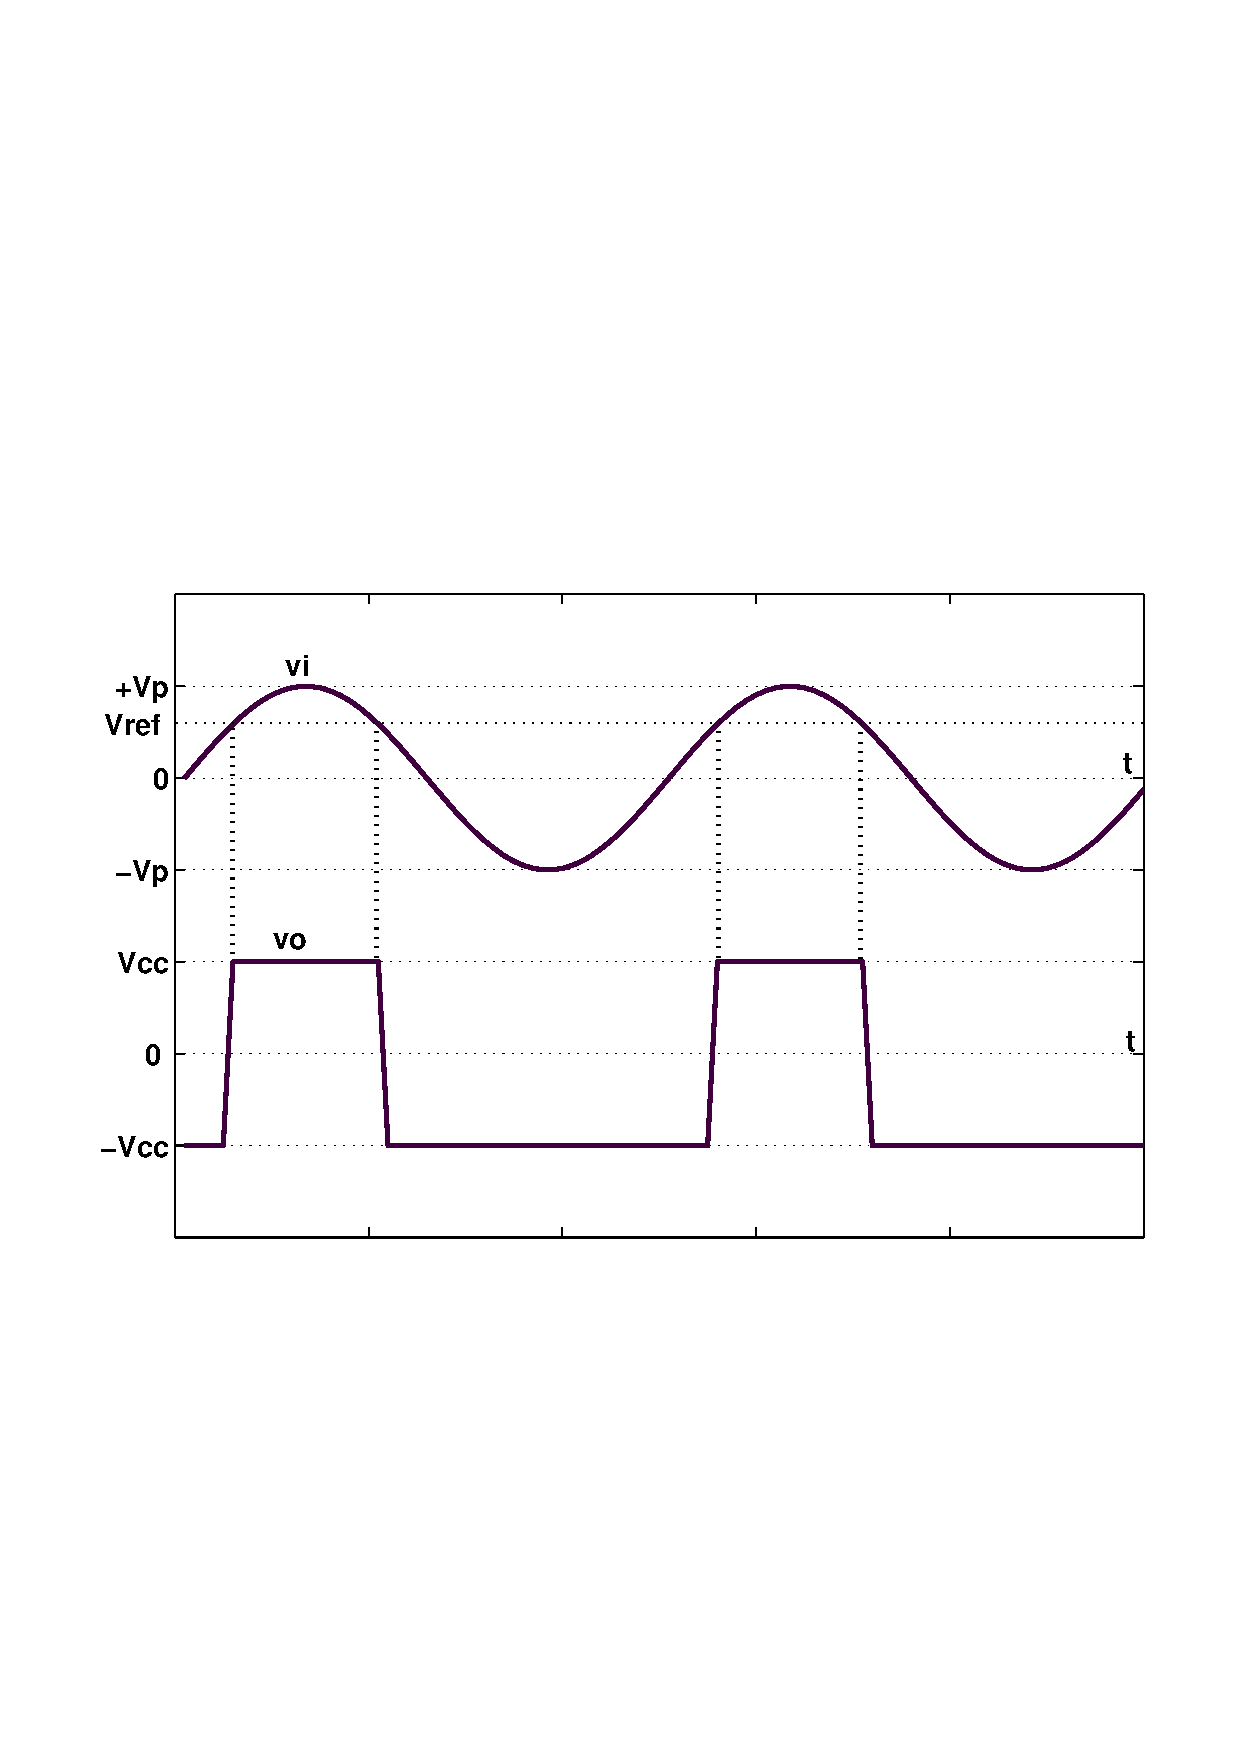
\includegraphics[width=3in]{figuras/ao35.png}\\
	\caption{Respuesta de un comparador no inversor a una onda senoidal.}\label{ao35}
\end{figure}

\begin{figure}
	\centering
	\includegraphics[width=2.5in]{figuras/ao36.png}\\
	\caption{Comparador no inversor ajustable.}\label{ao36}
\end{figure}

\subsection{Comparador con histéresis (Schmitt Trigger)}

\hspace{10pt} El comparador desarrollado en el punto anterior posee un único
umbral de comparación. Cuando la entrada llega al umbral,
la salida cambia de valor. Si hay ruido superpuesto con la señal de
entrada, puede haber una oscilación transitoria en la salida hasta
que la señal de entrada más el ruido superpuesto superen al valor
umbral.

Para evitar esta indeterminación se utiliza un comparador con
histéresis eléctrica, es decir un comparador con dos umbrales de
comparación lo suficientemente alejados para evitar el efecto del
ruido.

Para lograrlo se utiliza un comparador realimentado positivamente,
como  el mostrado en el circuito de la figura \ref{ao37} a) denominado comparador con
histéresis o \textbf{Schmitt Trigger}, que posee una transferencia
diferente de acuerdo al sentido de variación de la entrada. Para
comprender su funcionamiento analizaremos el caso en que $v_i=0V$, y
supondremos que la salida se encuentra saturada en $+V_{CC}$; esta
situación estable es una de las dos posibles, siendo la otra posible
que $v_o=-V_{CC}$ cuando $v_i=0V$. En el primer caso se puede
demostrar que $V^+=V_{CC}\frac{\displaystyle
	R_2}{\displaystyle R_1+R_2}+V_{ref}\frac{\displaystyle
	R_1}{\displaystyle R_1+R_2}=V_{U1}$, siendo este valor el umbral de
comparación para el caso en que $v_o=+V_{CC}$; en la figura
\ref{ao37} b) se muestra la transferencia de este caso en el que se
encuentra aumentando $v_i$, allí se ve que cuando $v_i$ supera a
$V_{U1}$ la salida vuelca a $-V_{CC}$ y por lo tanto el umbral de
comparación cambia a $V^+=-V_{CC}\frac{\displaystyle
	R_2}{\displaystyle R_1+R_2}+V_{ref}\frac{\displaystyle
	R_1}{\displaystyle R_1+R_2}=V_{U2}$. Si partimos ahora del caso
$v_i=+V_{CC}$ y $v_o=-V_{CC}$ y siendo el umbral de comparación
$V_{U2}$, vemos que al disminuir $v_i$ se tiene la transferencia
mostrada en la figura \ref{ao37} c), cuando $v_i$ es menor que
$V_{U2}$ la salida vuelve a volcar a $+V_{CC}$ siendo nuevamente el
umbral de comparación $V_{U1}$. En la figura \ref{ao37} d) se
muestra la transferencia completa de acuerdo al sentido de variación
de $v_i$. Diseñando apropiadamente $R_1$, $R_2$ y $V_{ref}$ se
pueden lograr distintas posiciones y anchos de la ventana de
histéresis.
\begin{figure}
	\centering
	\includegraphics[width=2.5in]{figuras/ao37.png}\\
	\caption{Comparador con histéresis Schmitt Trigger. a) Esquema circuital, b) transferencia para $v_i$ incrementándose, c) transferencia para $v_i$ disminuyendo y d) transferencia total. }\label{ao37}
\end{figure}

\subsection{Generadores de señales con comparadores.}

\hspace{10pt} Utilizando comparadores se pueden diseñar una gran cantidad de
circuitos generadores de señales.

El circuito de la figura \ref{ao38} es un generador de onda
cuadrada. La realimentación positiva, predominante sobre la
negativa, hace que la salida del comparador trabaje en saturación
($\pm V_{cc}$). El umbral de comparación que produce los cambios en
la salida está dado por: $V_u=V^+=\pm V_{cc} \frac{\displaystyle
	R_1}{\displaystyle R_1+R_2}$.

En la figura \ref{ao38} se define a la tensión  $V_c=V^-$ como la
tensión en el capacitor, la tensión de salida $V_o$ y la tensión de
umbral $V^+$ ya definida anteriormente.

Para analizar el funcionamiento en el tiempo supondremos la
siguiente condición inicial en $t=0$: $V_c(0)=0V$ (capacitor
descargado) y $V_o(0)=+V_{cc}$. Por lo tanto
$V^+=+V_{cc}\frac{\displaystyle R_1}{\displaystyle R_1+R_2}$. Esta
condición de $V_o=+V_{cc}$ se sostendrá mientras que $V^+ > V^-$. Es
de notar que partiendo de condiciones iniciales distintas se llegará
al mismo funcionamiento en estado permanente. En la figura
\ref{ao39} se muestra la evolución temporal de $V_c(t)$ en línea
gruesa y de $V_o(t)$ en línea fina.

Bajo las condiciones iniciales ya mencionadas el capacitor $C$
comenzará a cargarse según el circuito $RC$ alimentado por
$V_o=+V_{cc}$, por lo tanto la tensión del capacitor ($V_c=V^-$)
será:
$$V_c(t)=V_{cc}(1-e^{\displaystyle -\frac{\displaystyle t}{\displaystyle \tau}})$$, con
$\tau=RC$. El capacitor aumentará su tensión hasta un tiempo $t_1$
en el cual su tensión se iguale con la tensión de comparación
$V^+=+V_{cc}\frac{\displaystyle R_1}{\displaystyle R_1+R_2}$, este
tiempo puede calcularse de:
$$V_c(t_1)=V_{cc}(1-e^{\displaystyle -\frac{\displaystyle t_1}{\displaystyle
		\tau}})$$, de aquí se deduce que:
$$t_1=\tau \ln {\frac {\displaystyle R_1+R_2}{\displaystyle R_2}}$$. Un infinitésimo después
($t_1^+$) el comparador ideal volcará
instantáneamente hacia $V_o=-V_{cc}$ debido a que el capacitor posee
una tensión infinitesimalmente mayor a $V^+$ sin poderla variar
instantáneamente. La nueva situación en $t'=t-t_1$ será:
$V_o=-V_{cc}$, $V^+=-V_{cc}\frac{\displaystyle R_1}{\displaystyle
	R_1+R_2}$ y $V_c(t'=0)=V_{cc}\frac{\displaystyle R_1}{\displaystyle
	R_1+R_2}$. En estas condiciones el capacitor se descargará según la
expresión:
$$V_c(t')=-V_{cc}+(V_{cc}\frac{\displaystyle R_1}{\displaystyle
	R_1+R_2}+V_{cc})e^{\displaystyle -\frac{\displaystyle
		t'}{\displaystyle \tau}}$$, en $t'=t_2$ el capacitor alcanzará la
tensión de umbral $-V_{cc}\frac{\displaystyle R_1}{\displaystyle
	R_1+R_2}$, dicho tiempo se calcula con:
$$V_c(t_2)=-V_{cc}\frac{\displaystyle R_1}{\displaystyle
	R_1+R_2}=-V_{cc}+(V_{cc}\frac{\displaystyle R_1}{\displaystyle
	R_1+R_2}+V_{cc})e^{\displaystyle -\frac{\displaystyle
		t_2}{\displaystyle \tau}}$$, se deduce que:
$$t_2=\tau \ln {\frac {\displaystyle 2R_1+R_2}{\displaystyle R_2}}
$$. La salida del comparador volcará ahora a $V_o=+V_{cc}$, el
umbral de comparación pasará a $V^+=+V_{cc}\frac{\displaystyle
	R_1}{\displaystyle R_1+R_2}$ y la tensión inicial del capacitor será
$V_c=-V_{cc}\frac{\displaystyle R_1}{\displaystyle R_1+R_2}$. Con
consideraciones similares al caso anterior y suponiendo
$t''=t'-t_2$, se llega a que el capacitor se cargará siguiendo a:
$$V_c(t'')=V_{cc}+(-V_{cc}\frac{\displaystyle R_1}{\displaystyle
	R_1+R_2}-V_{cc})e^{\displaystyle -\frac{\displaystyle
		t''}{\displaystyle \tau}}$$, hasta un tiempo $t_3$ en que
nuevamente alcance al umbral de comparación, por simetría se ve que $t_3=t_2$. Este comportamiento se
repetirá indefinidamente alternando carga y descarga del capacitor
dando a la salida una forma de onda cuadrada como puede apreciarse
en la figura \ref{ao39}.

\begin{figure}
	\centering
	\includegraphics[width=2.5in]{figuras/ao38.png}\\
	\caption{Generador de onda cuadrada con comparador. }\label{ao38}
\end{figure}

\begin{figure}
	\centering
	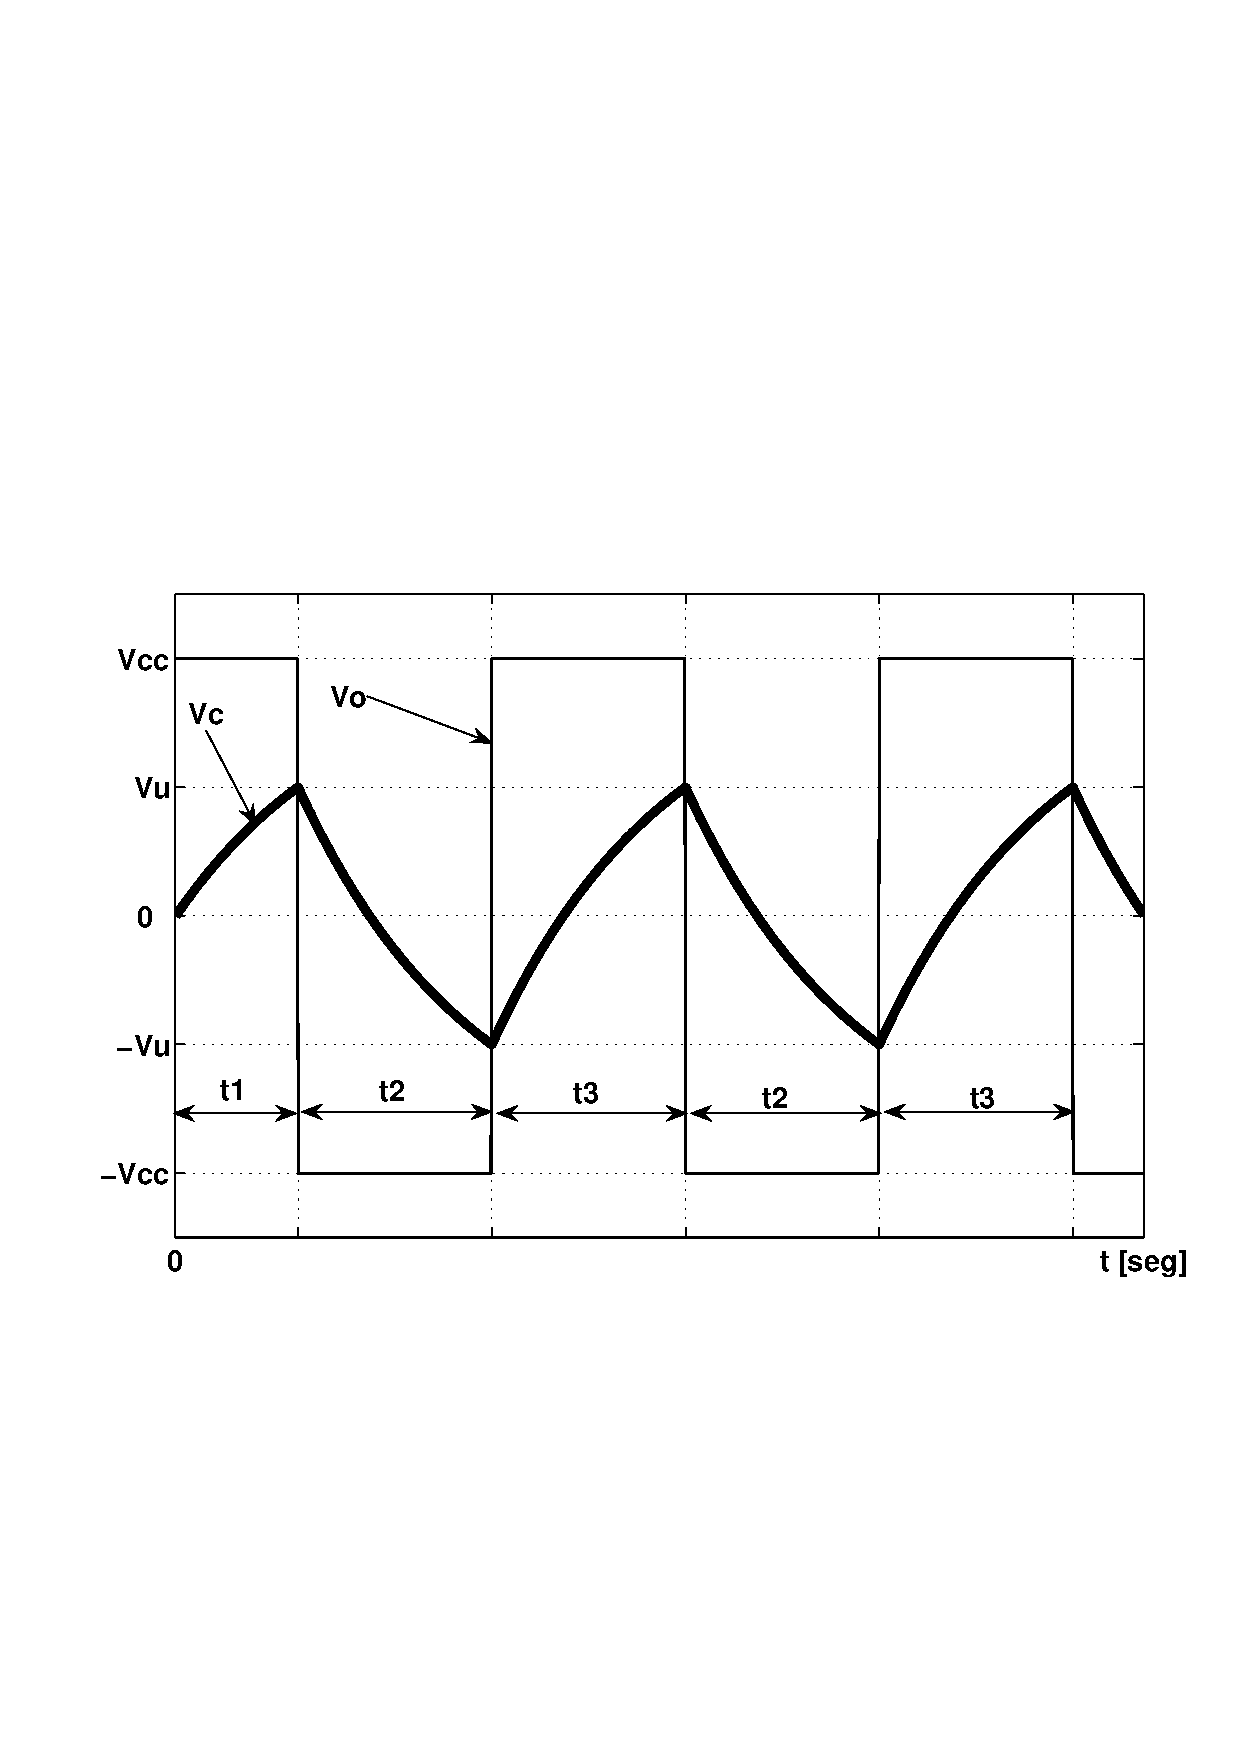
\includegraphics[width=4.5in]{figuras/ao39.png}\\
	\caption{Formas de onda de $V_c$ y $V_o$ para el generador de onda cuadrada.}\label{ao39}
\end{figure}

Otro ejemplo de generador de señales utilizando comparadores es el
mostrado en la figura \ref{ao40}. En dicha figura el amplificador
denominado \textbf{a1} trabaja como comparador con realimentación
positiva. Cuando la tensión en el nodo \textbf{$V_x$} es mayor que
0V su salida será $V_{o1}=+V_{CC}$, cuando es menor que 0V será
$V_{o1}=-V_{CC}$. El amplificador \textbf{a2} trabaja con
realimentación negativa como un integrador inversor, por lo tanto si
la señal $V_{o1}$ es cuadrada la salida $V_o$ será triangular. Para
verificar este comportamiento, y partiendo del circuito de la figura
\ref{ao40}, se plantean las siguientes expresiones:

$$V_o(t)=V_C(t)=-\frac{\displaystyle 1}{\displaystyle RC}\int_0^t V_{o1}(t)dt +V_o(0)$$

$$V_x(t)=\frac{\displaystyle V_{o1}(t)}{\displaystyle 3}+2 \frac{\displaystyle V_{o}(t)}{\displaystyle 3}$$

Si se parte de la condición inicial $V_C(0)=V_o(0)=0V$ y
$V_{o1}(0)=+V_{CC}$ se obtiene para el primer tramo de
funcionamiento las siguientes expresiones:

$$V_o(t)=-\frac{\displaystyle V_{CC}}{\displaystyle RC} t$$

$$V_x(t)=\frac{\displaystyle V_{CC}}{\displaystyle 3}-\frac{\displaystyle V_{CC}}{\displaystyle RC}\frac{\displaystyle 2}{\displaystyle 3} t$$

En la figura \ref{ao41} se grafican $V_{o1}$, $V_o$ y $V_x$ en
función del tiempo.

En el tiempo $t_1$ la tensión $V_x(t_1)=0V$, en esta condición la
salida del comparador \textbf{a1} vuelca a $V_{o1}=-V_{CC}$,
invirtiéndose el sentido de carga del capacitor. El tiempo $t_1$ se
calcula de: $V_x(t_1)=0V=\frac{\displaystyle V_{CC}}{\displaystyle
	3}-\frac{\displaystyle V_{CC}}{\displaystyle RC}\frac{\displaystyle
	2}{\displaystyle 3} t_1$, dando $t_1=\frac{\displaystyle
	RC}{\displaystyle 2}$.

A partir de este momento, suponiendo un origen en $t'=t-t_1$ y
teniendo en cuenta que $V_o(t'=0)=-\frac{\displaystyle
	V_{CC}}{\displaystyle 2}$ se obtienen las siguientes expresiones de
funcionamiento:

$$V_o(t')=-\frac{\displaystyle V_{CC}}{2}+\frac{\displaystyle V_{CC}}{\displaystyle RC} t'$$

$$V_x(t')=-2\frac{\displaystyle V_{CC}}{\displaystyle 3}+\frac{\displaystyle V_{CC}}{\displaystyle RC}\frac{\displaystyle 2}{\displaystyle 3} t'$$

En $t'=t_2$ la tensión $V_x$ pasará nuevamente por $0V$, la salida
del comparador \textbf{a1} volcará a $V_{o1}=V_{CC}$. De esta
condición se deduce que:  $t_2=RC$.

Si corremos nuevamente el origen a $t''=t'-t_2$ y consideramos que
$V_o(t''=0)=\frac{\displaystyle V_{CC}}{\displaystyle 2}$ el
funcionamiento estará dado por:

$$V_o(t'')=\frac{\displaystyle V_{CC}}{2}-\frac{\displaystyle V_{CC}}{\displaystyle RC} t''$$

$$V_x(t'')=2\frac{\displaystyle V_{CC}}{\displaystyle 3}-\frac{\displaystyle V_{CC}}{\displaystyle RC}\frac{\displaystyle 2}{\displaystyle 3} t''$$

En $t''=t_3$ la tensión $V_x$ pasará nuevamente por $0V$, la salida
del comparador \textbf{a1} volcará a $V_{o1}=-V_{CC}$. De esta
condición se deduce que:  $t_3=t_2=RC$.

Este comportamiento se repetirá indefinidamente alternando carga y
descarga del capacitor dando las formas de onda que pueden
apreciarse en la figura \ref{ao41}.


\begin{figure}
	\centering
	\includegraphics[width=3.5in]{figuras/ao40.png}\\
	\caption{Generador de onda triangular y cuadrada. }\label{ao40}
\end{figure}

\begin{figure}
	\centering
	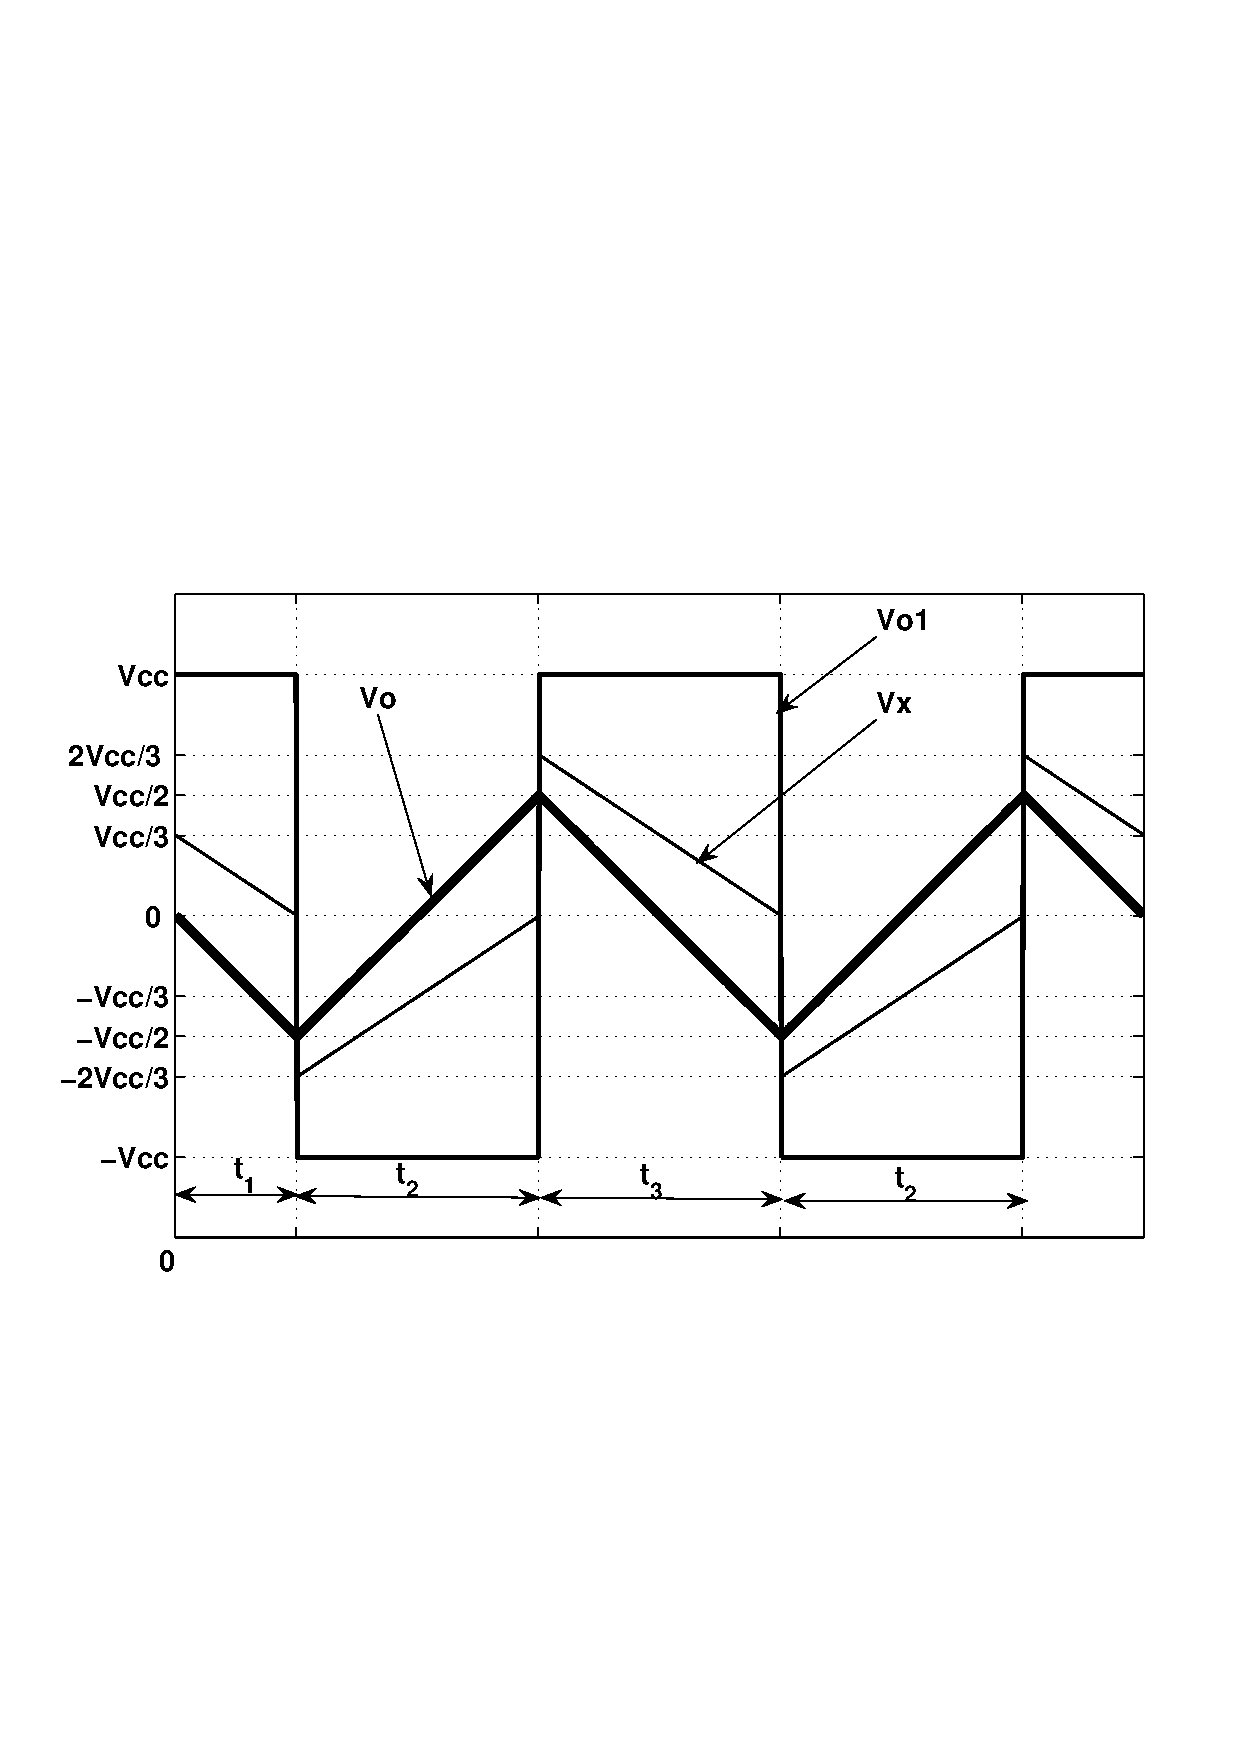
\includegraphics[width=4.5in]{figuras/ao41.png}\\
	\caption{Formas de onda de $V_o$, $V_x$ y $V_{o1}$ para el generador de onda triangular y cuadrada.}\label{ao41}
\end{figure}
